\documentclass[11pt]{article}
\usepackage{graphicx}
\usepackage{amsmath}
\usepackage{listings}
\graphicspath{ {./} }
\setcounter{secnumdepth}{0}

\begin{document}
\begin{titlepage}
   \begin{center}
       \vspace*{1cm}
       \textbf{\Huge Numerical Methods} \\
       \vspace{2.0cm}
       \huge{ProjectAssignment B: Nonlinear algebraic equations} \\
       \vspace{.7cm}
       \huge{\today} \\
       \vspace{3.0cm}
       \vspace{0.4cm}
       Krzysztof Watras\\
       \vspace{ 0.2cm }
       \small{ Tutor's name: Jakub Wagner } \\
       \vspace{2 cm}   
       \small{Computer Science} \\  
       \vspace{0.2cm}       
       \small{Warsaw University of Technology,\\
       Faculty of Electronics and Technology} \\
       \vspace{2cm}
       \small{I declare that this piece of work, which is the basis for
       recognition of achieving learning outcomes in the Numerical Methods
       course, was completed on my own. Krzysztof Watras} \\
   \end{center}
\end{titlepage} 
\tableofcontents

\newpage
\section{Introduction}
In this report I analyze the difference between methods of finding the
solutions to nonlinear algebraic equations. By solving the equation I mean
finding such $x$ such that $f(x) = 0$. I will compare methods given by
comparing them to \textbf{fzero} function as a reference method built-in to
MATLAB language. Function that I use in the report is the following:
\begin{equation}
    f(x) = 2.5\cdot \cos^3(-\frac{x}{7}-1.5) - 0.01\cdot
    \left(\frac{x}{3}\right)^3 + 2 
    \mbox{, where } x \in [0,10]
\end{equation}

Function is visualized on Figure~\ref{fig:functionplot}

\begin{figure}[ht!]
    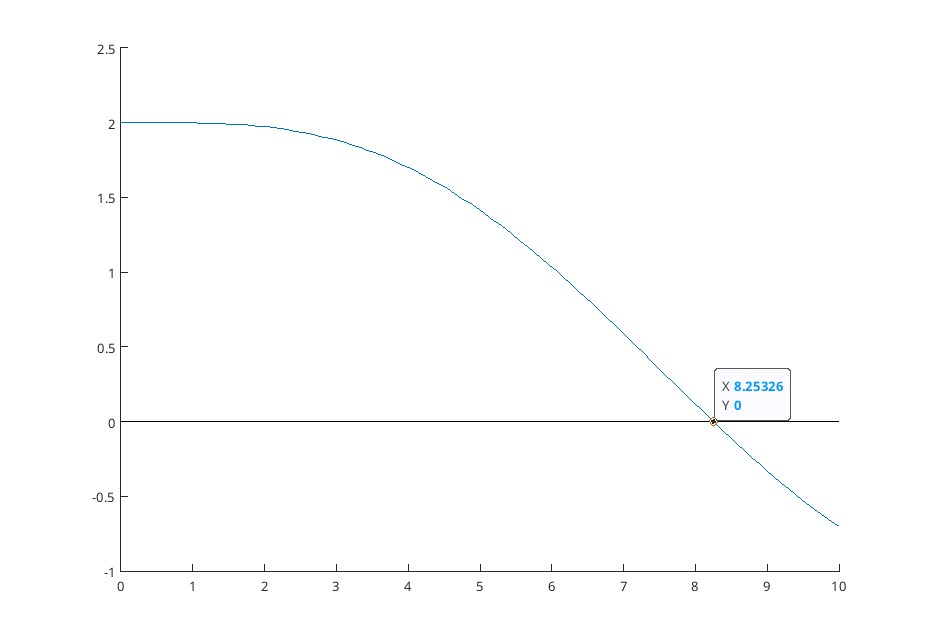
\includegraphics[width=\textwidth]{Function_plot.jpg}
    \caption{Function f(x) and the intersection with the y=0}
    \label{fig:functionplot}
\end{figure}

As one can clearly see, the intersection is found at the point $x=8.25326$.
This is verified by \textbf{fzero} function that returns $8.2533$ and after use
of \textit{format long} to increase number of digits displayed we get
$8.253263117902842$, which is consistent with the observation from the graph.

\newpage
All of my algorithms will use common interface to all: \\
As input arguments I'll use:
\begin{itemize}
    \setlength\itemsep{0em}
    \item \textbf{f} is a \textit{function handle} of function analyzed 
    \item \textbf{x} is a 2 element vector containing the start and end of the
        interval
    \item \textbf{xeps} is a maximal error that we allow this function to
        return
\end{itemize}
And the return will be a vector of consecutive solutions. This will allow for
easier testing as well as comparison between solutions.

Only exception from this standard will be Newton's method where \textbf{x}
represents the starting point for the algorithm. This is because newton's
method needs only one point to work.

When comparing the algorithms, the $\rho$ property will be stated. It is an
exponent of convergence and is a good measure that informs how quickly the
algorithm converges to the true correct value.

\newpage
\section{Bisection method}
Bisection method is an iterative algorithm used for finding roots of an
equation. It works by continuously splitting the initial interval into halves,
until the solution is found. Here, the exponent of convergence $\rho=1$.

My solution in code:
\lstinputlisting[language=MATLAB]{bisection.m}

This can be summarized by following steps:
\begin{enumerate}
    \setlength\itemsep{0em}
    \item Initialize variables
    \item Is maximal error smaller than the specified one? End if true
    \item Save result of current approximation to return vector
    \item Adjust interval accordingly
    \item Goto step 2
\end{enumerate}
We find max error by calculating $|\frac{a-b}{2}|$. If this error is below the
intended threshold we stop the algorithm. This is because in the worst case our
solution is only half of the interval length away from true root of the 
equation.

We verify that this with a graph of total error.
\begin{figure}[ht!]
    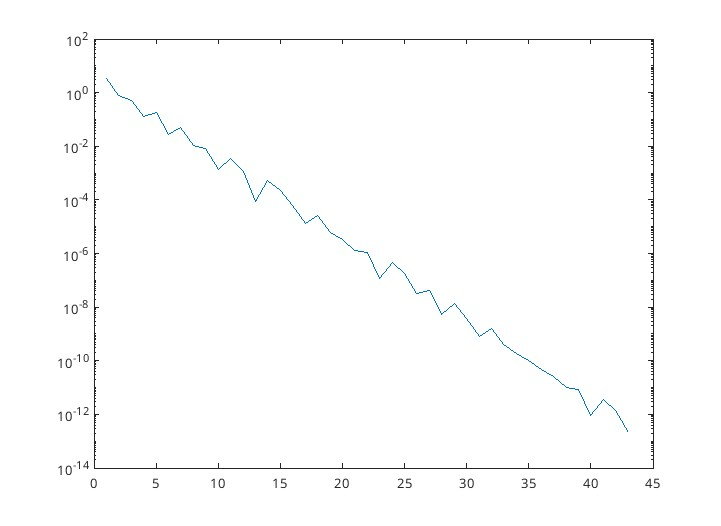
\includegraphics[width=\textwidth]{bisection_test.jpg}
    \caption{Absolute error in each iteration of bisection method}
    \label{fig:bisection_test}
\end{figure}
As one can clearly see, from Figure~\ref{fig:bisection_test}, the error indeed
goes down and algorithm stops around the expected $10^{-12}$ value of error.
Note: Algorithm does not stop exactly as the "true error" hits $10^{-12}$. This
is because algorithm does not know this "true error". Instead, it knows what is
the max error at each iteration. Hence, it continues to run for a couple more
iterations.

\newpage
\section{Secant Method}
The secant method is an iterative root-finding algorithm that uses
successive solutions of secant lines to approximate a root of a function f.
It has a $\rho=1.618$ or $\frac{\sqrt{5}+1}{2}$. 
Following equation describes the algorithm. 
$$x_{i+1} = x_i - \frac{x_i - x_{i-1}}{f(x_i)-f(x_{i-1})}$$
It is similar to the Newton-Raphson method, but instead of using the
derivative of the function, it uses a numerical approximation of the
derivative.

My solution in code:
\lstinputlisting[language=MATLAB]{secant.m}

This can be summarized by following steps:
\begin{enumerate}
    \setlength\itemsep{0em}
    \item Initialize variables
    \item Is maximal error smaller than the specified one? End if true
    \item Calculate the secant of point we are at
    \item Set variables for next iteration
    \item Goto step 2
\end{enumerate}

\newpage
\section{Newton's Method}
Newton's method is perhaps the most famous method of solving nonlinear equations.
It is very efficient method having a $\rho$ factor of 2.
It was also famously used in Fast Inverse Of Square Root algorithm by William Kahan [2].
Following equation describes the algorithm. 
$$x_{i+1} = x_i - \frac{f(x_i)}{f'(x_i)}$$

My solution in code:
\lstinputlisting[language=MATLAB]{newton.m}

This can be summarized by following steps:
\begin{enumerate}
    \setlength\itemsep{0em}
    \item Initialize variables
    \item Is maximal error smaller than the specified one? End if true
    \item Calculate the secant of point we are at
    \item Set variables for next iteration
    \item Goto step 2
\end{enumerate}

Note: In my implementation I use following property to calculate the derivative of function.
$$f'(x) = \frac{Imag(f(x + i\cdot \eps))}{\eps}$$
This was introduced to us during the consultations for this rapport. A good
paper on this property is "Using Complex Variables to Estimate Derivatives of
Real Functions" by Lyness and Moler, which was published in SIAM Journal on
Numerical Analysis in 1967 [3]. What is fascinating about this property is that
it works for calculating the first derivative of function, but does not
calculate the second derivative of the same function.

\newpage
\section{Muller's Method, second version}
The method is iterative, meaning it uses an initial guess and then improves
upon it with each iteration. The algorithm requires three initial guesses,
$x_0, x_1, \mbox{and } x_2$. Here we use $x_{min}, x_{avg}, \mbox{and }
x_{max}$ respectively. Muller Method has $\rho$ value equal to 1.84 so lower
that the Newton's method, but higher than secant method. 

Following equation describes the algorithm. 
$$ 
M = 
\begin{bmatrix} a_i \\ b_i \end{bmatrix} =
\begin{bmatrix} 
    -(x_i - x_{i-1})^2 & (x_i - x_{i-1}) \\
    -(x_i - x_{i-2})^2 & (x_i - x_{i-2})
\end{bmatrix}^{-1} \cdot 
\begin{bmatrix} 
    f(x_i) -f(x_{i-1}) \\
    f(x_i) -f(x_{i-2})
\end{bmatrix}
\mbox{, and } c_i = f(x_i)
$$
And then, the iterative formula is equal to 
$$x_i = x_i - \frac{2c_i}{b_i + sgn(b_i)\sqrt{b_i^2-4a_i c_i}}$$

My solution in code:
\lstinputlisting[language=MATLAB]{muler2.m}

\newpage
\section{Comparison of different methods}

\begin{figure}[ht!]
    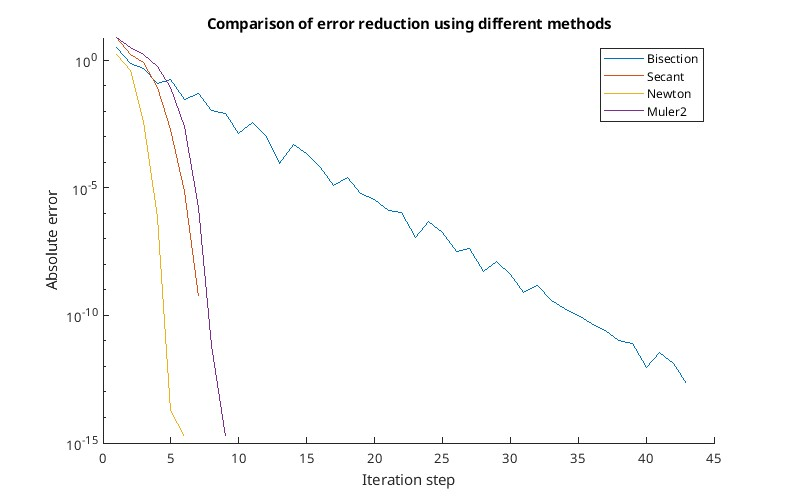
\includegraphics[width=\textwidth]{combined_test.jpg}
    \caption{Absolute error in each iteration of different methods}
    \label{fig:combinedtest}
\end{figure}

Figure~\ref{fig:combinedtest} shows the consecutive result error for each
algorithm. As one can see, the worst method in terms of number of iterations is
the bisection method. The best one was Newton's method. Secant and Muller
methods are comparable, though secant method performed better. This observation
is consistent with the $\rho$ properties of those algorithms. Newton's method
has highest value of $\rho$ and converges the fastest to true value. Bisection
method has lowest value of $\rho$ and converges the slowest to true value.
Secant method has $\rho$ comparable to Muller's method and has similar
convergence. However, it did perform better while calculating this particular
function, despite lower $\rho$ value. This is a good reminder that while
general rules are good guidelines, they are not definite and to be sure one
needs to test their solutions to be sure.

\begin{figure}[ht!]
    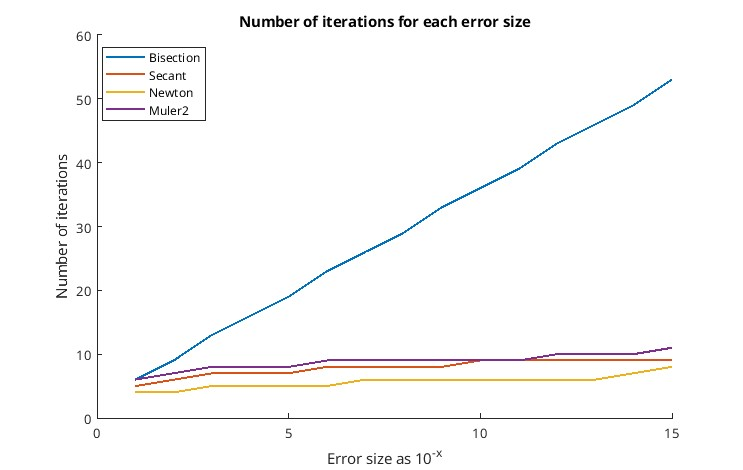
\includegraphics[width=\textwidth]{iter_per_error_size.jpg}
    \caption{Number of iterations needed to obtained result for each algorithm and error $\in [10^{-15}, 10^{-1}]$}
    \label{fig:iter_per_error_size}
\end{figure}

Crucially, the scalability of the algorithms is consistent with the results we
got in a single error size test. When testing the performance of algorithms
across errors $\in [10^{-15}, 10^{-1}]$ we can see which algorithms perform and
scale the best. This can be seen on Figure~\ref{fig:iter_per_error_size}.

\newpage
\section{Comparison of theoretical number of iterations and true iteration number in a bisection method}
For a bisection method an expected value of iterations is expressed by following formula.
$$I = log_2(\frac{|b-a|}{\delta})$$
which in our function is equal to 
$$I = log_2(\frac{10}{\Delta}) \mbox{, where } \Delta \in [10^{-15}, 10^{-1}]$$

\begin{figure}[ht!]
    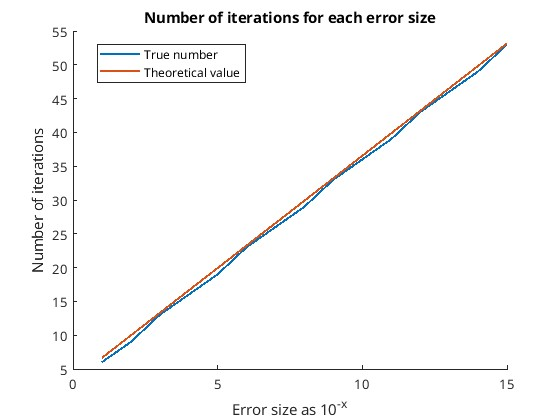
\includegraphics[width=\textwidth]{comp_theor_real.jpg}
    \caption{Comparison of true number of iterations and theoretical number needed}
    \label{fig:comparison6}
\end{figure}
As one can see on Figure~\ref{fig:comparison6}, the true number of iterations
closely follows the theoretical value that one should expect.

\newpage
\section{Comparison of convergence of Newton's method based on starting point}
Without code and simply knowing the function shape and how Newton's method
works we can assume that it'll take more iterations for it to converge when
starting on the left side of the interval. 

\begin{figure}
    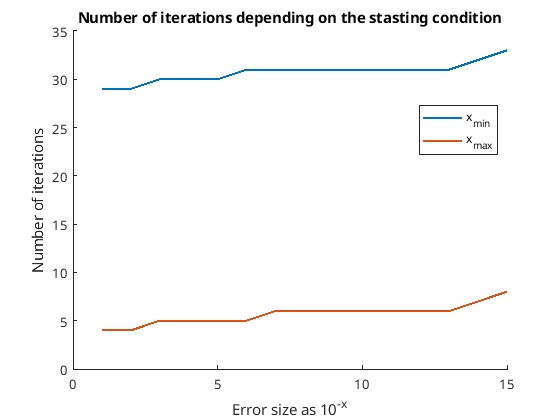
\includegraphics[width=\textwidth]{sol7.jpg}
    \caption{Comparison of iteration number depending on starting condition}
    \label{fig:sol7}
\end{figure}

Figure~\ref{fig:sol7} shows exactly what we would expect. 
The difference between results is rather big. This means that although the
algorithm is very efficient compared to others, it is beneficial to know what
initial value to set. 

\newpage
\section{References}
{[1]} R. Z. Morawski: Numerical methods (ENUME) – \emph{2. Accuracy and
complexity of computing}, Warsaw University of Technology, Faculty of
Electronics and Information Technology \\
{[2]} https://en.wikipedia.org/wiki/Fast_inverse_square_root \\
{[3]} https://epubs.siam.org/doi/10.1137/S003614459631241X \\

\newpage
\section{Appendix: Listing of the developed programs}
\subsection{Source code for Task 1}
\lstinputlisting[language=MATLAB]{sol1.m}
\newpage
\subsection{Source code for Task 4}
\lstinputlisting[language=MATLAB]{sol4.m}
\newpage
\subsection{Source code for Task 5}
\lstinputlisting[language=MATLAB]{sol5.m}
\subsection{Source code for Task 6}
\lstinputlisting[language=MATLAB]{sol6.m}
\newpage
\subsection{Source code for Task 7}
\lstinputlisting[language=MATLAB]{sol7.m}

\end{document}

